% !TeX spellcheck = en_US
\newpage
\section{Transport}
The transport layer operates in an \textbf{end-to-end} fashion, encapsulating the network layer. Its main goals are:
\begin{itemize}
	\item \textbf{End-to-End reliability}:
	\begin{itemize}
		\item \textit{Deliver}: guarantee that the packets sent are indeed delivered
		\item \textit{Order}: guarantee that the packets arrive in the order they were sent
	\end{itemize}
	\item \textbf{End-to-End flow control}: techniques to match the source sending rate with the destination receiving rate
	\item \textbf{Congestion control}: techniques to regulate sending rates of sources to \textbf{prevent network overload}
	\item \textbf{Multiplexing} and \textbf{demultiplexing} to allow sharing of an interface between multiple applications
\end{itemize}

\subsection{Basic elements}
\subsubsection{De/Multiplexing}
Since multiple applications share the same network interface, there is a need to multiplex and demultiplex between the applications and the network layer. This is done with \textbf{ports}: a networking abstraction that allows to identify applications. The port combined with the IP address is a \textbf{socket}: operating system abstraction that identifies processes to exchange network messages.

\begin{center}
	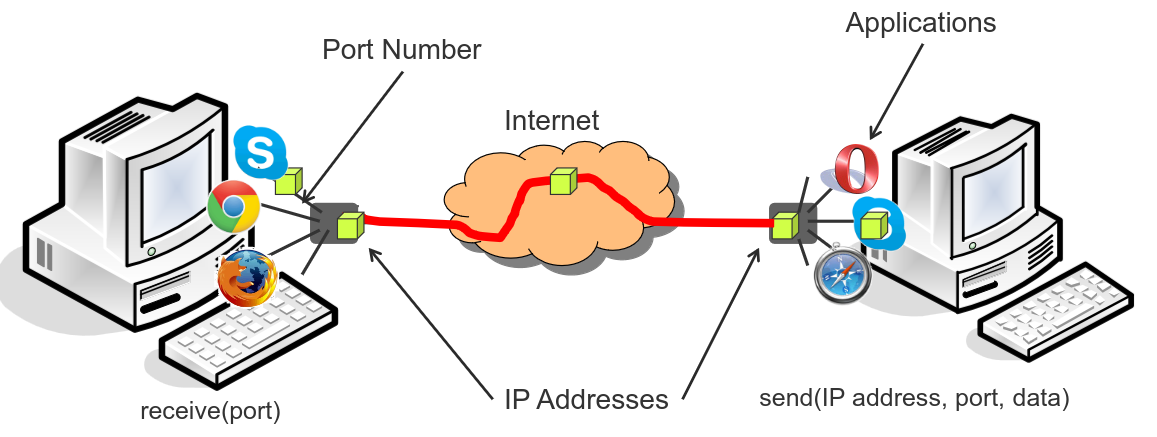
\includegraphics[scale=.3]{socket}
\end{center}
Port numbers are coded on 16 bits and are divided between:
\begin{itemize}
	\item \textbf{well-known}: from $0$ to $1023$, used by known services and assigned by IANA and IETF
	\item \textbf{registered}: from $1024$ to $49151$, assigned by IANA and used also by OS
	\item \textbf{dynamic/private}: from $49152$ to $65535$
\end{itemize}

\subsubsection{Primitives}
Transport layer provides:
\begin{itemize}
	\item \textbf{Unreliable datagram service} (connectionless)
	\item \textbf{\textbf{Reliable service}} (connection-oriented), divided in three phases:
	\begin{enumerate}
		\item \textit{Establishment}
		\item \textit{Communication}
		\item \textit{Termination}
	\end{enumerate}
\end{itemize}
\newpage \noindent The \textbf{primitives} for a \textit{connection-oriented} service are:
\begin{table}[!h]
	\centering
	\begin{tabular}{|c|c|c|}
		\hline
		\textbf{Primitive} & \textbf{Packet sent} & \textbf{Meaning} \\
		\hline
		\textit{LISTEN} & (none) & Block until some process tries to connect \\
		\hline
		\textit{CONNECT} & CONN REQ & Actively attempt to establish a connection \\
		\hline
		\textit{SEND} & DATA & Send information \\
		\hline
		\textit{RECEIVE} & (none) & Block until DATA packet arrives \\
		\hline
		\textit{DISCONNECT} & DISC REQ & This side wants to release connection \\
		\hline
	\end{tabular}
\end{table}

\paragraph{Establishment}
\begin{wrapfigure}[10]{r}{6cm}
	\vspace{-1cm}
	\begin{center}
		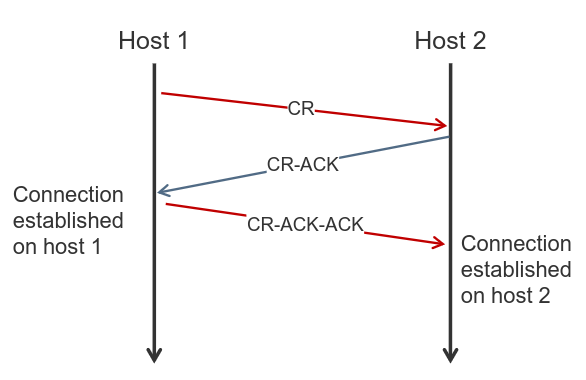
\includegraphics[width=6cm]{3way}
	\end{center}
\end{wrapfigure}
End-to-End communication setup is done with a \textbf{3-way handshake} so that the communication can be verified in both directions. \\\\
The main problem is \textbf{delayed duplicates}: we need to introduce a \textbf{sequence number} so that identically numbered transport packets are never out at the same time for different connections between hosts. Each connection will start numbering with a different initial sequence number.\\\\
If a delayed duplicate Connection Request arrives at host it gets rejected since it doesn't recognize the sequence number.

\paragraph{Termination} There are two types of releases:
\begin{itemize}
	\item \textbf{Asymmetric}: either one peer terminates the connection
	\item \textbf{Symmetric}: both peers have to terminate the connection explicitly
\end{itemize}
Both approaches could cause \textbf{data loss}. Thus a \textbf{timer} is introduced: it starts when a Disconnect Request is sent, if it timeouts the request is sent again and the connection is terminated abruptly only after $N$ failed tries.

\begin{figure}[!h]
	\centering
	\subfigure[Normal case]{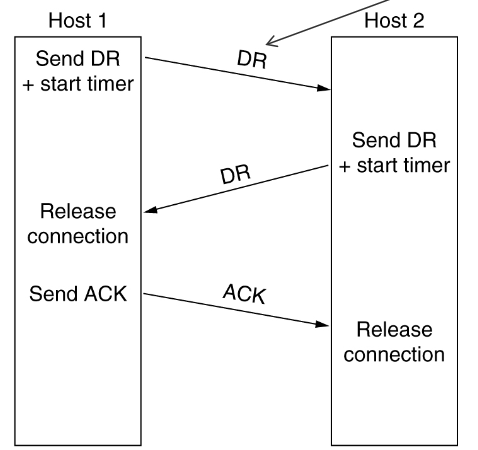
\includegraphics[scale=0.25]{term1}}
	\hfil
	\subfigure[Final ACK lost]{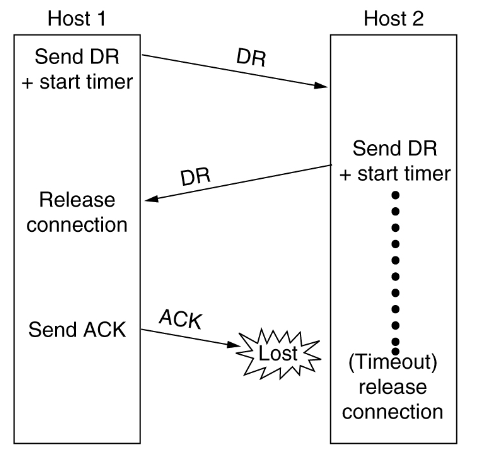
\includegraphics[scale=0.25]{term2}}\\
	\subfigure[Response lost]{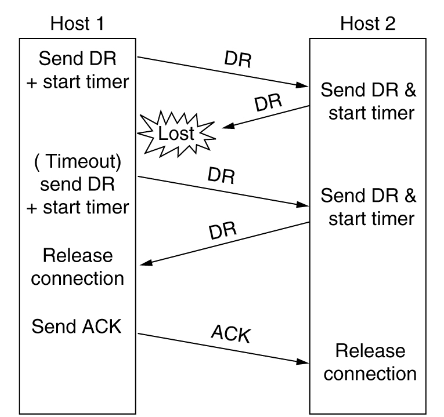
\includegraphics[scale=0.25]{term3}}
	\hfil
	\subfigure[Response and DRs lost]{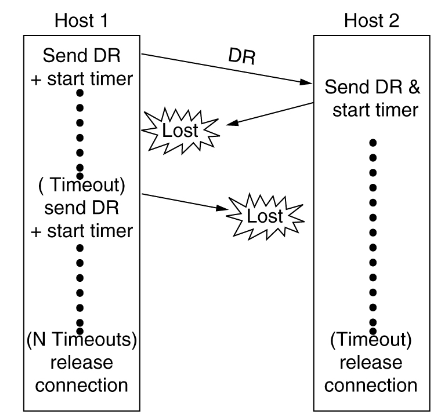
\includegraphics[scale=0.25]{term4}}
\end{figure}

\paragraph{Crash recovery} If both hosts and routers are subject to crashes, recovery becomes an issue, e.g. a client sends a large file to a server, each chunk is ACKed but after a crash the server doesn't know the status.\\
In particular, a client could be in two \textbf{states}:
\begin{enumerate}
	\item \textbf{No} outstanding ACK
	\item \textbf{Outstanding} ACK
\end{enumerate}
It has four possible strategies:
\begin{itemize}
	\item Always retransmit last packet
	\item Never retransmit last packet
	\item Retransmit last packet in state (1)
	\item Retransmit last packet in state (2)
\end{itemize}
On the other hand the server has two possible strategies in case of a  crash (C):
\begin{itemize}
	\item First send ACK (A), then write (W) to application
	\item First write to application, then send ACK
\end{itemize}
The different combination of the possible client/server strategies lead to different scenarios:
\begin{center}
	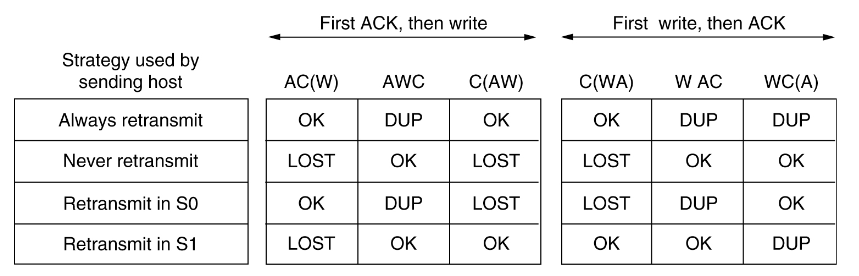
\includegraphics[scale=.4]{crash}
\end{center}

\subsection{Protocols}
\subsubsection{UDP}
The \textbf{User Datagram Protocol} follows the \textbf{KISS} (keep It Simple Stupid) principle. It uses a small 8 byte header and it's \textbf{connectionless} and \textbf{unreliable}, but \textbf{fast}.\\
There is no acknowledgment between peers: incorrect packets are discarded, there is only a basic checksum and duplicates/loss/packet permutations are possible.

\begin{center}
	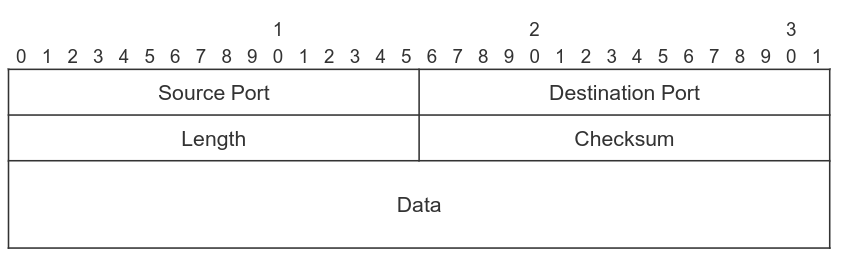
\includegraphics[scale=.3]{udp}
\end{center} 
\begin{itemize}
	\item \textbf{Source} and \textbf{destination port}: addressing of the applications by port number
	\item \textbf{Length}: total length of the datagram in 32 bits word
	\item \textbf{Checksum}, optional
	\item \textbf{Data}: the payload, filled up if necessary to an even byte number since the length is in 32bit words
\end{itemize}
The main \textbf{reasons} to choose UDP are:
\begin{itemize}
	\item \textbf{Multiplexing}: the tuple (port, network address) uniquely identifies end-points
	\item \textbf{Control}: application has finer-grain control, useful for real-time communication
	\item \textbf{Speed}: no delay due to connection establishment
	\item \textbf{Statelessness}: small packet header
	\item \textbf{Multicasting}
\end{itemize}

\subsubsection{TCP}
\textbf{Transmission Control Protocol} is: \textbf{point-to-point} (one sender, one receiver), \textbf{full duplex}, \textbf{connection-oriented}, \textbf{reliable}, \textbf{flow} and \textbf{congestion controlled} and \textbf{pipelined}.\\
It sends and receives segments to establish and terminate a connection, agree on a window size and transmit data.
\begin{center}
	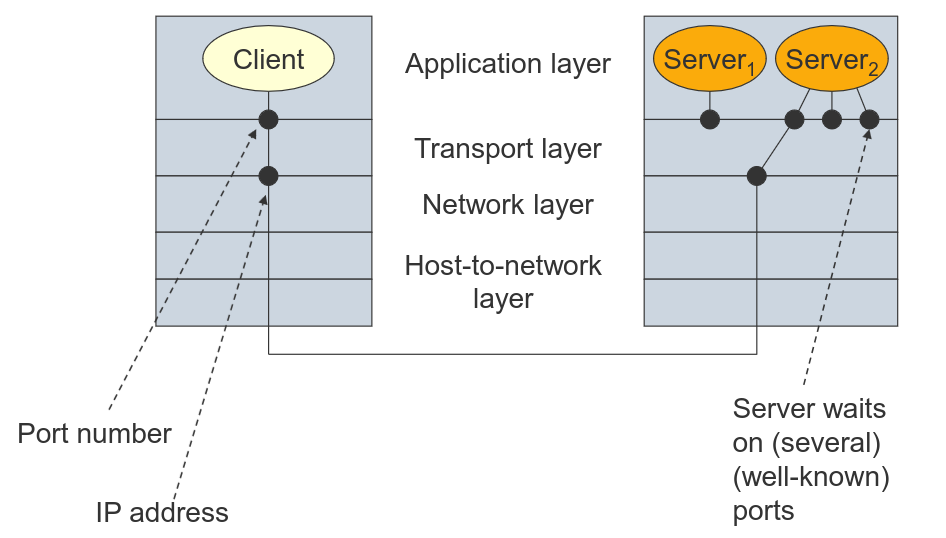
\includegraphics[scale=.3]{tcp}
\end{center}

\paragraph{Header} TCP has a 20 bytes header that supports plus options and up to 65495 data bytes.
\begin{center}
	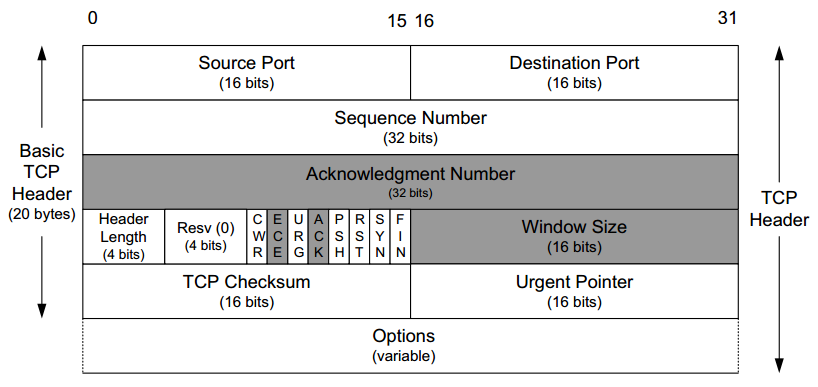
\includegraphics[scale=.4]{tcpheader}
\end{center}
\begin{itemize}
	\item \textbf{Source} and \textbf{destination port}: port number of sender and receiver
	\item \textbf{Sequence} and {acknowledgment number}: they're used for the window mechanism in flow control (\textbf{Sliding Window}). The first indicates the sequence number of the first data byte in this segment and they are random initialized. The second indicates the next expected byte and acks all prior ones.
	\item \textbf{Header Length}: length of the header in terms of 32 bit words with a minimum of $5$ and a maximum of $15$
	\item \textbf{Window Size}: size of the receiver's buffer for the connection. The window indicates how many bytes at the same time can be sent.
	\item \textit{Flags}
	\begin{itemize}
		\item \textbf{Congestion Window Reduced}: set by a sender to inform a receiver that the congestion window has been reduced
		\item \textbf{ECE}: indicates an ECN-Echo, it's set by a receiver to inform the sender that it received a packet with ECN set in the IP header, meaning that it experienced congestion. If \textbf{SYN} is set, indicates that a TCP peer is ECN capable
		\item \textbf{URG}: signaling of important data, e.g. CTRL+C
		\item \textbf{ACK}: set if it's an acknowledgment
		\item \textbf{PSH}: immediate transmission of data without waiting for further data
		\item \textbf{RST}: reset a connection e.g. during a crash
		\item \textbf{SYN}: set to $1$ for connection \textit{establishment}
		\item \textbf{FIN}: set to $1$ for connection \textit{termination}
	\end{itemize}
	\item \textbf{Urgent Pointer}: if \textit{URG} is set, indicates at which position in the data field the urgent data ends through a byte offset of the current sequence number
	\item \textbf{Options}, some of them are:
	\begin{itemize}
		\item Negotiation of a \textbf{window scale}, allowing window size field to be shifted up to 14 bits
		\item Use of \textbf{Selective Repeat} instead of Go-Back-N in case of an error
		\item Indication of the \textbf{Maximum Segment Size} to determine the size of the data field
	\end{itemize}
	\item \textbf{Checksum}: classical use and also verifies that the packet was delivered to the right host. It's computed using a \textbf{pseudo header}
	\begin{center}
		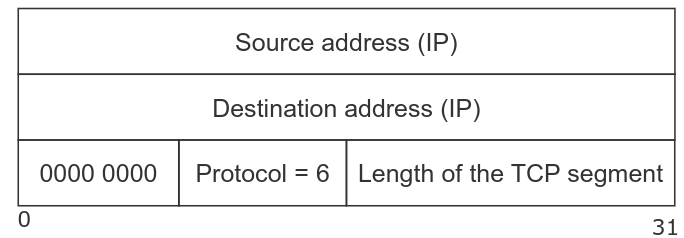
\includegraphics[scale=.3]{pseudoheader}
	\end{center}
	which is put in front of the main header. The checksum is then computed as the 1-complement of the sum of all 16-bit words of the segment, including the pseudo header.
\end{itemize}

\paragraph{Connection management} A connection is divided in three phases:
\begin{enumerate}
	\item \textbf{Establishment}: the server waits for connection requests with \textbf{LISTEN}. The client uses \textbf{CONNECT} and specifies IP address, port and MSS and sends them setting the SYN flag. If the server accepts through \textbf{ACCEPT}, it returns a segment with SYN and ACK flags. The client then sends back a segment with the ACK flag.
	\item \textbf{Data Transmission}: it's a \textbf{full-duplex} connection where a byte stream is segmented. All hosts must accept at least segments of 556 bytes. Segments up to ACK-1 are confirmed and if there is a timeout before an ACK, the sender repeats, either with \textit{Go-Back-N} o\textit{Selective Repeat}.
	\item \textbf{Termination}: a segment with the FIN flag is sent, if it gets confirmed that direction is switched off but the opposite one remains open and data can be still be sent
\end{enumerate}
\begin{center}
	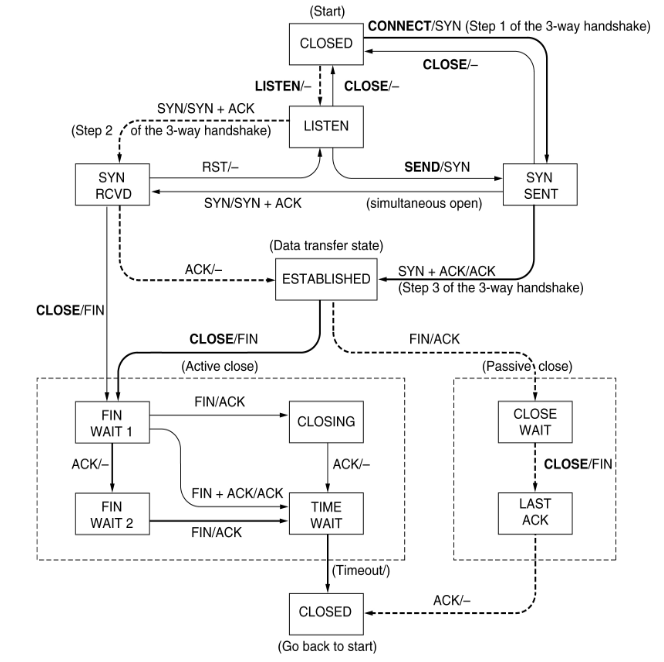
\includegraphics[scale=.5]{tcpfsm}
	\captionof{figure}{Finite state machine of a TCP connection}
\end{center}
\paragraph{Timer management} TCP uses several timers to schedule \textbf{retransmissions}. They are computed by estimating the probability density of the RTT and setting $T > RTT$. If the timer is too small, there are too many retransmissions but if it's too large there is a big delay to recover from packet loss.\\
\textbf{SampleRTT} is the average of several recent measurements of time from segment transmission until ACK receipt. There are two algorithms to handle the retransmission timer:
\begin{itemize}
	\item \textbf{Jacobson}: TCP manages a variable RTT that holds the best current estimation of the round trip time. When sending a segment a timer is started to measure the time needed for the ACK. If it arrives before the timeout , RTT is updated as follows
	\begin{equation}
		\text{RTT} = \alpha \cdot \text{RTT} + (1 - \alpha) \cdot \text{sampleRTT} \qquad\qquad \alpha=0.875
	\end{equation}
	The \textbf{timeout} was originally $\beta \cdot RTT$, with $\beta = 2$, but that was not reactive enough and was later redefined proportionally to the standard deviation of the arrival time of ACK
	\begin{equation*}
		\text{devRTT} = \gamma \cdot \text{devRTT} + (1-\gamma) \cdot \lvert \text{RTT} - \text{sampleRTT}\rvert \qquad\qquad \gamma = 0.75
	\end{equation*}
	and thus
	\begin{equation}
		\text{Timeout} = \text{RTT} + 4 \cdot \text{devRTT}
	\end{equation}
	\item \textbf{Karn}: do not update RTT on any segments that have been retransmitted. Timeout is doubled on each failure until the segments get through.
\end{itemize}
Other timers exist:
\begin{itemize}
	\item \textbf{Persistence}: prevents a deadlock with a loss of the buffer release message of a receiver. If the timer expires, the sender transfers a test segment. The response contains the current buffer size of the receiver. If it's still $0$ the timer starts again
	\item \textbf{Keep-Alive}: if a connection is alive for too long, at the end of the timer the other side is checked whether it's still alive. If not, the connection is terminated.
	\item \textbf{Time Wait}: during the termination of a connection, he timer runs for the double packet lifetime to be sure that no more late packets arrive
\end{itemize}

\paragraph{Reliable Transfer Management} TCP creates reliable data transfer service on top of IP’s unreliable service. It uses \textbf{retransmissions}, which are triggered either by:
\begin{itemize}
	\item \textbf{Timeout}: for every segment, start a timer and transmit it. If timeout occurs, retransmit the segment and restart the timer. There are three scenarios:
	\begin{itemize}
		\item \textbf{Lost ACK}: a segment arrives, ACK gets sent but gets lost, the segment is then retransmitted
		\item \textbf{Premature timeout}: segments arrive and ACKs are sent back correctly but too late, retransmission begins and with the first response all previous correctly received messages are ACKed
		\item \textbf{Cumulative ACK}: multiple segments arrive but the first ACK message gets lost, send an ACK message confirming all previous correctly received segments 
	\end{itemize}
	\begin{figure}[!h]
		\centering
		\subfigure[Lost ACK]{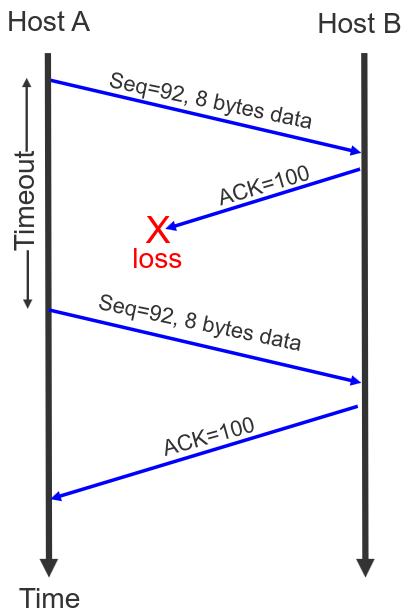
\includegraphics[scale=.2]{lost}}
		\subfigure[Premature timeout]{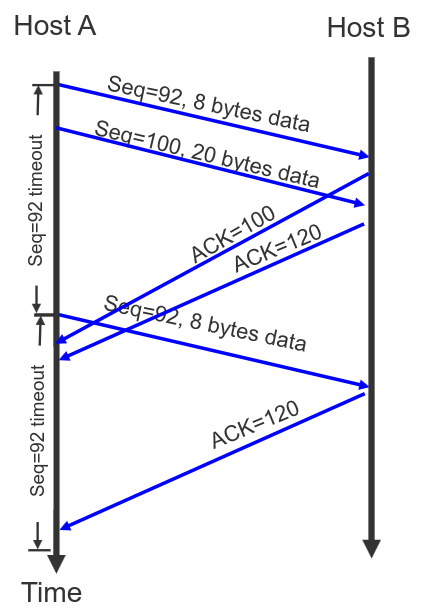
\includegraphics[scale=.2]{premature}}
		\subfigure[Cumulative ACK]{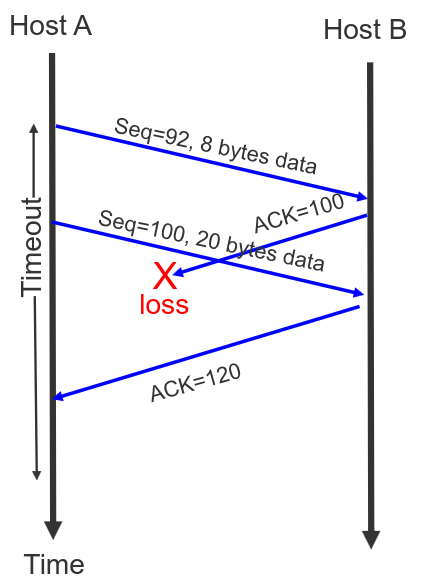
\includegraphics[scale=.2]{cumulative}}
	\end{figure}
	\begin{lstlisting}
		NextSeqNum = InitialSeqNum
		SendBase = InitialSeqNum
		loop (forever) {
			switch(event)
			event: data received from application above
			create TCP segment with sequence number NextSeqNum
			if (timer currently not running)
			start timer
			pass segment to IP
			NextSeqNum = NextSeqNum + length(data)
			event: timer timeout
			retransmit not-yet-acknowledged segment with smallest sequence number
			start timer
			event: ACK received, with ACK field value of y
			if (y > SendBase) {
				SendBase = y
				if (there are currently not-yet-acknowledged segments)
				start timer
			}
		}
	\end{lstlisting}
	\item \textbf{Duplicate ACKs}: when the same ACK is received multiple times, it's very likely that an intermediate segment got lost and needs to be resent
\end{itemize}
\newpage\noindent
ACK generation is done by the following rules:
\begin{table}[!h]
	\centering
	\def\arraystretch{1.5}
	\begin{tabular}{p{4cm}|p{4cm}}
		\textbf{Event at Receiver} & \textbf{TCP Receiver action} \\
		\hline
		Arrival of in-order segment with expected SEQNUM. All data up to that already ACKed & \textbf{Delayed ACK}, wait at least $500$ms for the next segment. If none arrives, send ACK. \\
		\hline
		Arrival of in-order segment with expected SEQNUM. One other has ACK pending & Immediately send single cumulative ACK, ACKing all in-order segments.\\
		\hline
		Arrival of out-of-order segment with higher than expected SEQNUM. Gap detected. & Immediately send \textbf{duplicate ACK} indicating SEQNUM of next expected byte \\
		\hline
		Arrival of segment that partially or completely fills the gap & Immediately send ACK, provided that segment starts at lower end of gap
	\end{tabular}
\end{table}

\paragraph{Flow control} To provide reliable data transfer, a \textbf{sliding window} mechanism is used: sender sends bytes according to the window size and the window gets shifted by $n$ bytes as soon as an ACK for those arrives. The window size can be changed dynamically during the transmission.
\begin{center}
	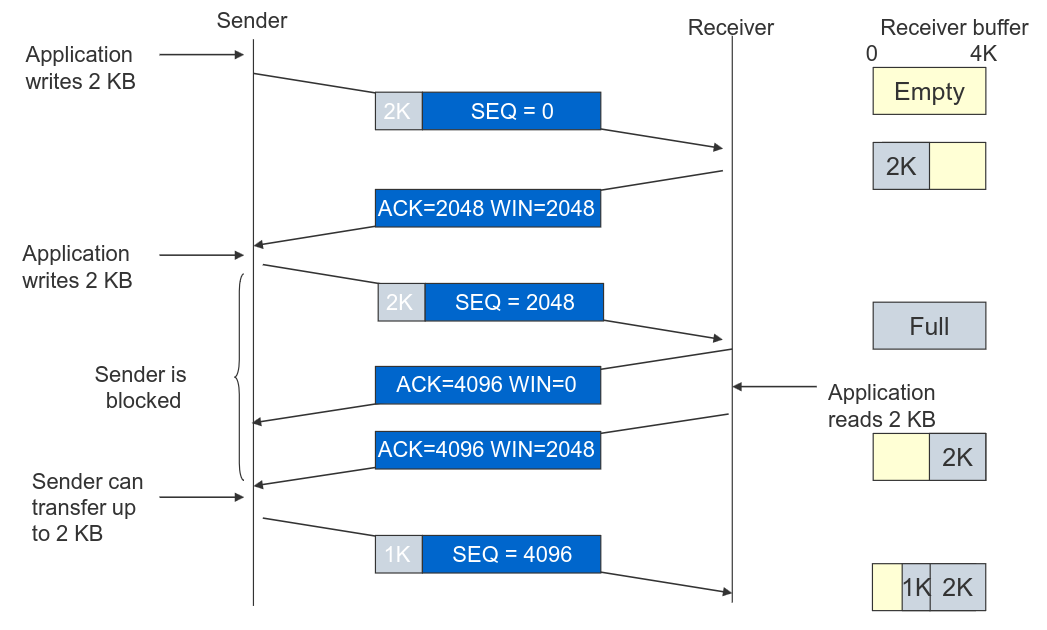
\includegraphics[scale=.3]{slidewin}
\end{center}
\begin{note}
	Urgent data is sent immediately disregarding the sliding window mechanism.
\end{note}

\paragraph{Congestion control} When too many sources send too much data too fast for the network to handle it, \textbf{congestion} happens. It manifests trough \textbf{long delays} and \textbf{lost packets}.\\
Endpoints do not know about congestion, they just experience it. If a timeout happens, the host retransmits the packets	leading to more traffic, more delay and so on.\\\\
Congestion control aims at solving three problems:
\begin{itemize}
	\item \textbf{Bandwidth estimation}: how to adjust the bandwidth of a single flow to the bottleneck bandwidth
	\item \textbf{Bandwidth adaptation}: how to adjust the bandwidth of a single flow to variation of the bottleneck bandwidth
	\item \textbf{Fairness}: how to share bandwidth fairly among flows, without overloading the network
\end{itemize}

\subparagraph{Detect} There are two main approaches to detect congestion:
\begin{itemize}
	\item \textbf{Network-Assisted}, through \textbf{Explicit Congestion Notification}: when supported by both endpoints (ECT flag), IP packets that traverse congested ares can be marked by routers. When the packet gets to the receiver, it echoes it back to signal that the sending rate should be reduced. The sender confirms that by setting the CWR flag.
	\item \textbf{End-to-End}: detecting losses can be done in two ways
	\begin{itemize}
		\item \textbf{Duplicated ACKs}: mild congestion signal, packets are still making it through
		\item \textbf{Timeout}: severe congestion signal, multiple consequent losses
	\end{itemize}
	This approach cannot distinguish between congestion or loss on link layer, which can be problematic in wireless communication.
\end{itemize}

\subparagraph{React} Sender throttles transmission with the minimum between the congestion and the receiver window
\begin{equation*}
	\text{LastByteSent} - \text{LastByteAcked} \leq \min(\text{CongWin}, \text{ReceiverWin})
\end{equation*}
Usually $\text{CongWin} < \text{ReceiverWin}$. The first one is dynamic and it's based on detection of loss events (timeout or 3 duplicate ACKs).
\begin{equation*}
	\text{rate} = \frac{\text{CongWin}}{\text{RTT}} \frac{\text{bytes}}{\text{sec}}
\end{equation*}
The regulation of CongWin can be done with different mechanisms:
\begin{itemize}
	\item \textbf{Additive Increase Multiplicative Decrease}: increase CongWin by $1$ \textbf{Maximum Segment Size} every RTT until loss detected, in that case cut it in half
	\item \textbf{Slow Start}:
	\begin{enumerate}
		\item Initialize CongWin to $1$ MSS and ReceiverWin to the value specified by the other end
		\item A segment with MSS bytes of data is sent
		\item Apply \textbf{Slow Start Algorithm}: when an ACK arrives before the time out, double CongWin, otherwise reset it to $1$ MSS. The growth stops when it reaches the flow control window size
	\end{enumerate}
	\item \textbf{Congestion avoidance} with \textbf{Inferring Loss}: introduce a threshold \textbf{ssthresh}, initialized at $64$ kbyte. Above ssthresh, CongWin increases linearly by $1$ MSS. In case of timeout, ssthresh is set to half of the maximum window size reached before it and CongWin is set to $1$ MSS.\\
	After $3$ duplicate ACKs, CongWin is halved and the windows then grows linearly
	\begin{center}
		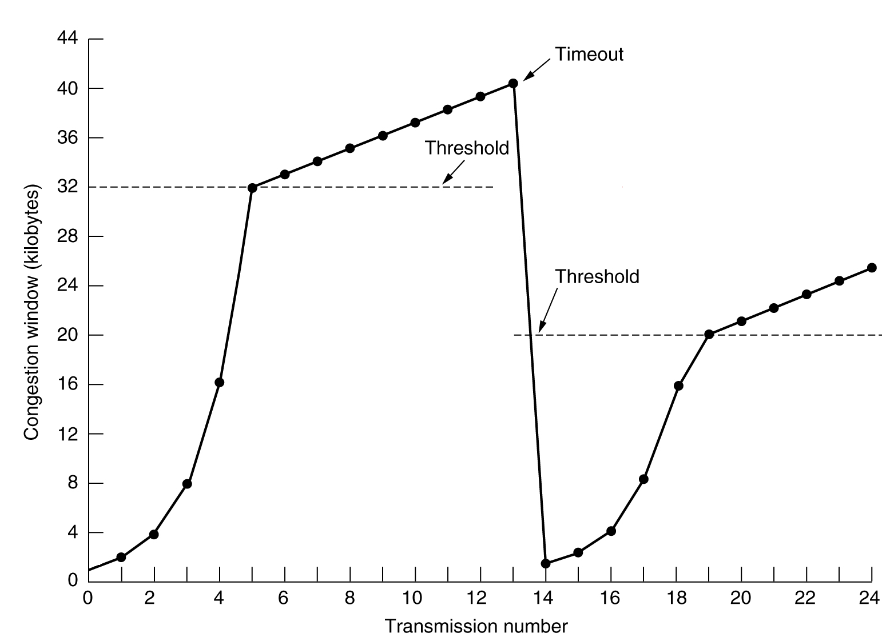
\includegraphics[scale=.3]{inferloss}
	\end{center}
	\item \textbf{Fast Retransmit and Recovery}: when a single packet is lost, Slow Start is not well suited. With Fast \textbf{Retransmit} the receiver sends duplicate ACKs immediately when out-of-order segments arrive. If the sender receives triple duplicate ACKs, it retransmits the missing segment, avoiding a new slow start phase.\\
	With Fast \textbf{Recovery}:
	\begin{enumerate}
		\item When the third ACK is received $\text{ssthresh} = \max(\frac{\text{ssthresh}}{2}, 2 \cdot \text{MSS})$
		\item Retransmit the  missing segment and set $\text{CongWin} = \text{ssthresh} + 3 \cdot \text{MSS}$
		\item For each subsequent duplicate ACK, increase CongWin by $1$ MSS
		\item If timeout happens, go back to slow start
	\end{enumerate}
\end{itemize}

\paragraph{Throughput}
\begin{wrapfigure}[12]{r}{4.5cm}
	\vspace{-1cm}
	\begin{center}
		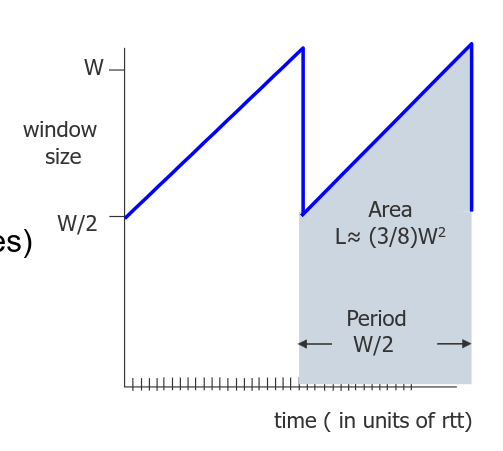
\includegraphics[width=4.5cm]{tp}
	\end{center}
\end{wrapfigure}
Given a \textit{window size}, the \textit{MSS}, the \textit{RTT} and the \textit{packet loss rate} $P$. Assuming no Slow Start, infinitely long TCP flow and periodic losses. The throughput of TCP is:
\begin{equation*}
	B = \frac{\text{Average number of bytes sent per cycle}}{\text{Average duration of a cycle}}
\end{equation*}
Since by definition each period delivers $\frac{1}{p}$ segments of MSS bytes and the total number of segments ACKed is the are under the saw tooth
\begin{equation*}
	\bigg(\frac{W}{2}\bigg)^2 + \frac{1}{2}\bigg(\frac{W}{2}\bigg)^2 = \bigg(\frac{3}{8}\bigg)W^2 \Longrightarrow W=\sqrt{\frac{8}{3W}}
\end{equation*}
Hence
\begin{equation}
	B = \frac{\text{MSS} \cdot \frac{3W^2}{8}}{\text{RTT}\cdot \frac{W}{2}} = \frac{\frac{\text{MSS}}{p}}{\text{RTT} \cdot \sqrt{\frac{2}{3p}}} = \frac{\text{MSS} \cdot C}{\text{RTT} \cdot \sqrt{p}} \qquad\qquad C = \sqrt{\frac{3}{2}}
\end{equation}

\paragraph{Fairness} If $k$ flows share the same bottleneck link of bandwidth $R$, each one of them should have an average rate of $\frac{R}{k}$. There are two approaches:
\begin{itemize}
	\item \textbf{Max-Min}: aims to give each session equal access to each link's bandwidth
	\item \textbf{Proportional}: if packet loss is \textit{synchronized} in different flows, there are times when the capacity is under-utilized, which is fair to no one. \textbf{Random Early Detection} in routers, tracks how the buffers fill up. If a buffer threatens to fill up soon, the router begins randomly dropping packets
\end{itemize}
Fairness can be difficult to achieve also because of \textbf{cheating}, misbehaving TCP flows, and \textbf{cohabitation} with non TCP traffic. 

\paragraph{Wireless} Transport layer protocols should be independent of lower layers, but TCP is optimized for wired networks since in wireless ones packet losses occur to other causes (hand off, bigger delays). For these reasons, TCP \textbf{performance} is very \textbf{poor} in wireless network. A few approaches to this problem are:
\begin{itemize}
	\item \textbf{Split-connection} TCP: the end-to-end connection is broken in two parts
	\item \textbf{Modifications} of TCP, which may lead to compatibility issues
	\item \textbf{New protocols}
\end{itemize}

\paragraph{Security} One of the attacks that can be performed on TCP is \textbf{SYN Flood}, which is a type of \textbf{Denial of Service}.\\\\
During connection establishment the client does not finish the three-way-handshake procedure and leaves a half open connection with the server still reserving resources. If this is repeated many times the server can be clogged.\\\\
A possible solution is using \textbf{SYN Cookies}: the server does not create a half-open connection. It computes an initial sequence number $y$ (the \textbf{cookie}) based on a hash function. When the client returns with ACK, the server checks again with the hash function and only then creates the connection.

\subsection{Newer protocols}
\begin{center}
	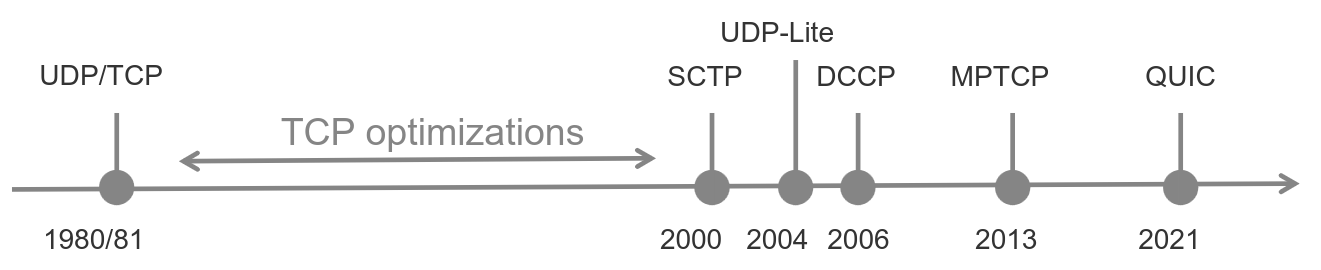
\includegraphics[scale=.25]{tranprot}
\end{center}
Choosing a transport protocol depends on the type of application: many of the new ones are driven by increased \textbf{readability}, reduced \textbf{latency} and \textbf{privacy}.\\
As of today, $85\%$ of IPv4 and $90\%$ of IPv6 traffic goes through TCP: there is an \textbf{ossification} of the transport layer, increasing the challenge to develop new protocols.\\\\
While originally protocols were focused on the end-to-end communication because we had dumb network and smart end devices, today it's not the same anymore: now we have as many \textbf{middleboxes} of different types as routers.
\begin{center}
	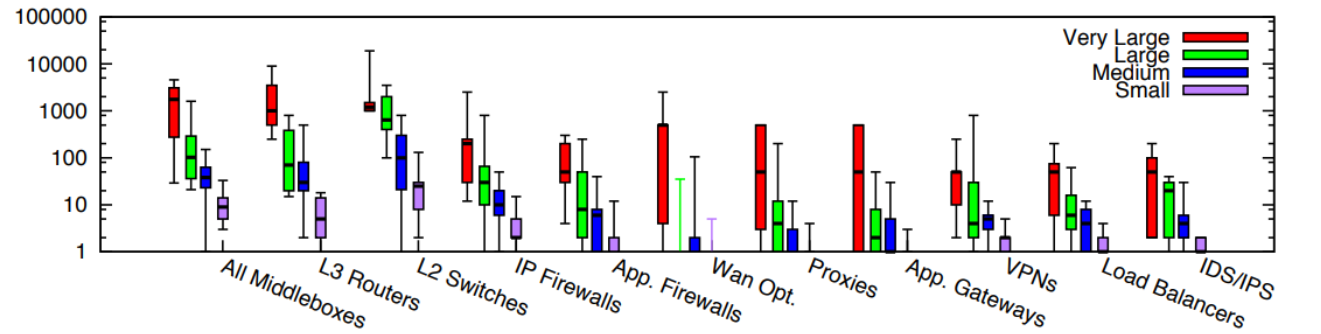
\includegraphics[scale=.2]{middleboxes}
\end{center}
Middleboxes are the new core problem:
\begin{itemize}
	\item They \textbf{assume} the format of the protocol header, making changes almost impossible
	\item They \textbf{modify some fields} of the transport or network layer, meaning that they cannot arrive at destination
	\item \textbf{Restrict} the usage of protocol extension that they don't support
\end{itemize}

\subsubsection{MPTCP}
\textbf{MultiPath TCP} was developed to increase reliability, efficiency and flexibility by exploiting multiple paths based on different IP addresses of the host and quickly moving traffic from congested or failed links.\\\\
It's based on the idea of \textbf{Resource Pooling}: making a collection of resources behave like a single pooled one.
\begin{wrapfigure}[10]{r}{4cm}
	\vspace{2.5cm}
	\begin{center}
		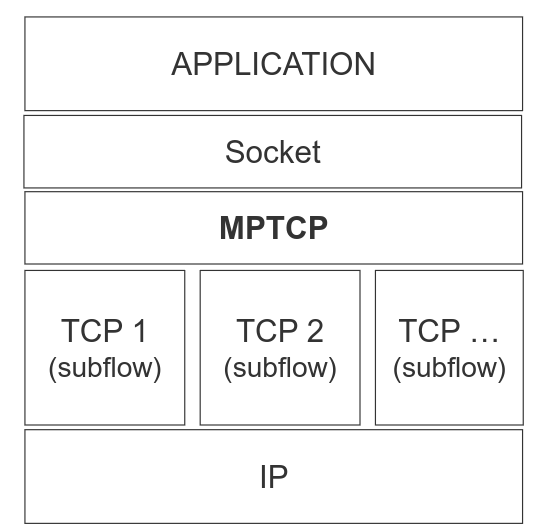
\includegraphics[width=4cm]{mtcp}
	\end{center}
\end{wrapfigure}
\begin{center}
	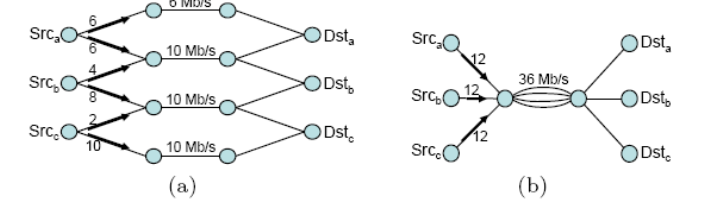
\includegraphics[scale=.3]{respool}
\end{center}

An MPTCP connection is composed of one or more regular TCP \textbf{subflows} that are combined. Each host maintains a state that glues them together. Each subflow is sent over a single path and appears like a regular TCP connection along it.\\
At least one of the following elements must differ between two subflows:
\begin{itemize}
	\item Local IP address
	\item Remote IP address
	\item Local port
	\item Remote port
\end{itemize}
\newpage
\begin{note}
	Number of subflows can change during the lifetime of an MPTCP connection.
\end{note}

\paragraph{Connection establishment} MPTCP connection establishment uses TCP mechanisms:
\begin{center}
	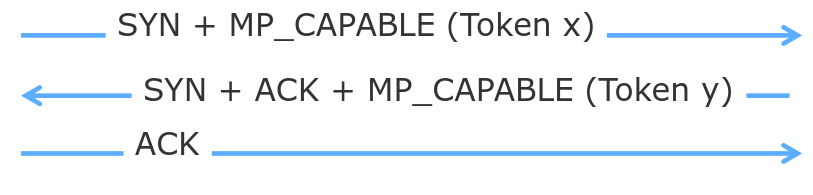
\includegraphics[scale=.3]{mptcpest}
\end{center}
\paragraph{Subflow start}
\begin{center}
	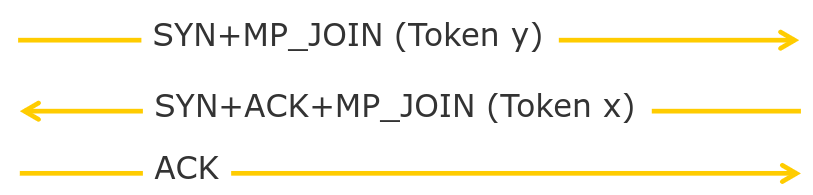
\includegraphics[scale=.3]{mptcpsub}
\end{center}
\paragraph{Data transfer} Since in today's internet there are many middleboxes, to transfer data MPTCP uses two level of sequence numbers:
\begin{itemize}
	\item \textbf{Data}: numbers the bytes in the \textit{byte stream}
	\item \textbf{TCP}: numbers the bytes inside the \textit{subflow}
\end{itemize}
Hence, regular TCP ACK confirms segments per subflows, while \textbf{DNS\_ACK} implements cumulative ACK per data sequence and prevents deadlock in case of proactive ACKs from middleboxes.
\begin{center}
	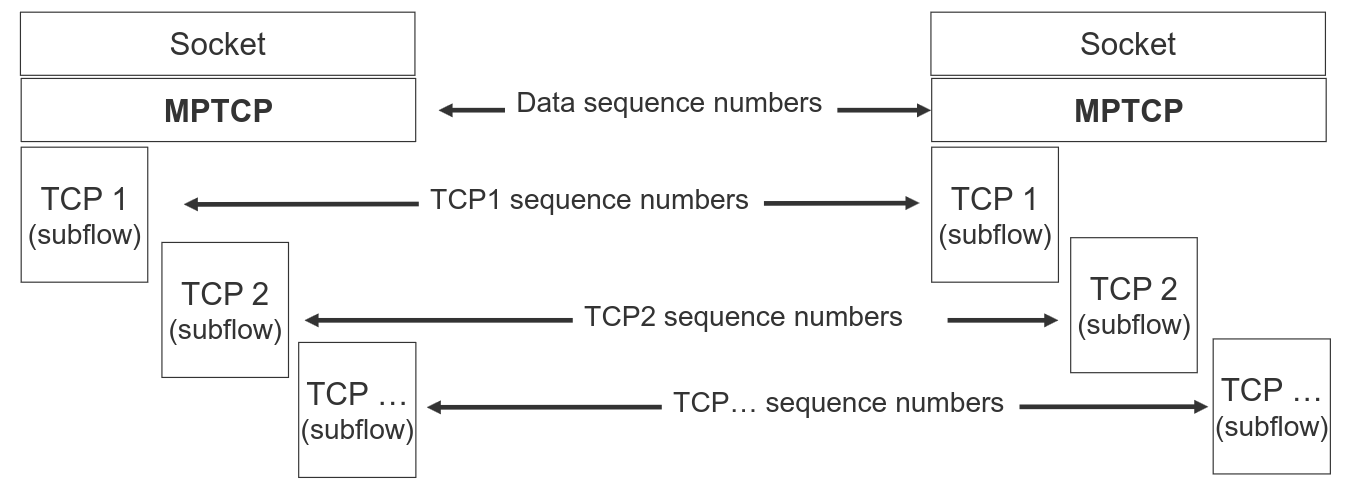
\includegraphics[scale=.25]{mptcpnum}
\end{center}
\begin{center}
	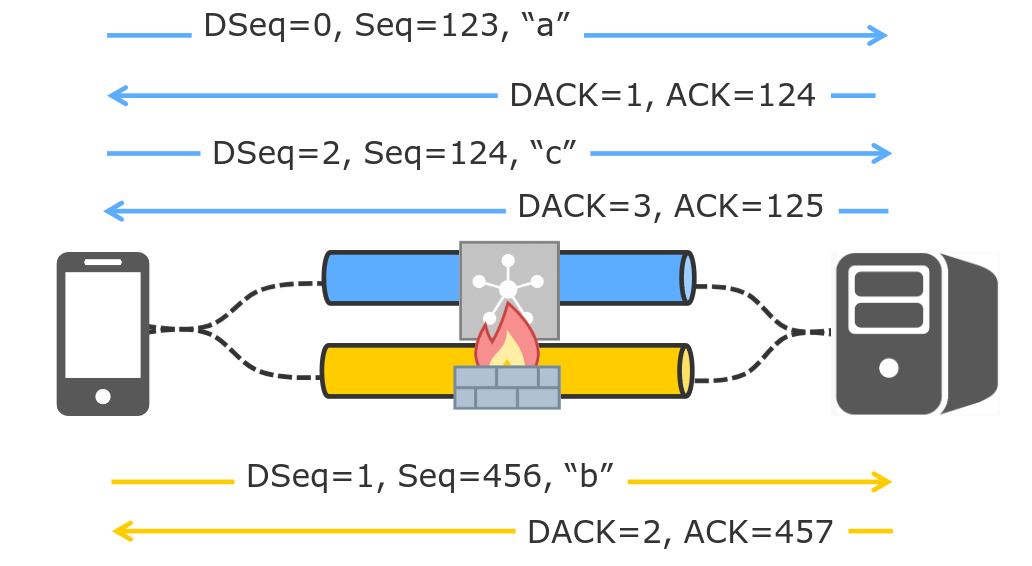
\includegraphics[scale=.3]{mptcptran}
\end{center}

\begin{observation}[Losses]
	When losses happen in a subflow, the subflow is completely lost.
\end{observation}

\subsubsection{QUIC}
The main reasons for QUIC are:
\begin{itemize}
	\item \textbf{Multiplexing}: for example, HTTP runs over TCP. HTTP/2 implemented full pipelining which is interfered by TCP: one lost packet in a stream requires all streams on the application layer to wait for successful retransmission. A simple solution is to run the protocol over UDP and improve connection management.
	\item \textbf{Surveillance}: implements minimal meta-data about the connection, reducing the ossification problem but making life more difficult for the providers
\end{itemize}
So overall the objectives are:
\begin{itemize}
	\item Easy deployment
	\item Low latency connection setup
	\item Multi-streaming
	\item Better security
	\item More efficient loss recovery and congestion control
	\item Multipath for resilience and load balancing
\end{itemize}

\begin{wrapfigure}[9]{r}{5cm}
	\vspace{-1cm}
	\begin{center}
		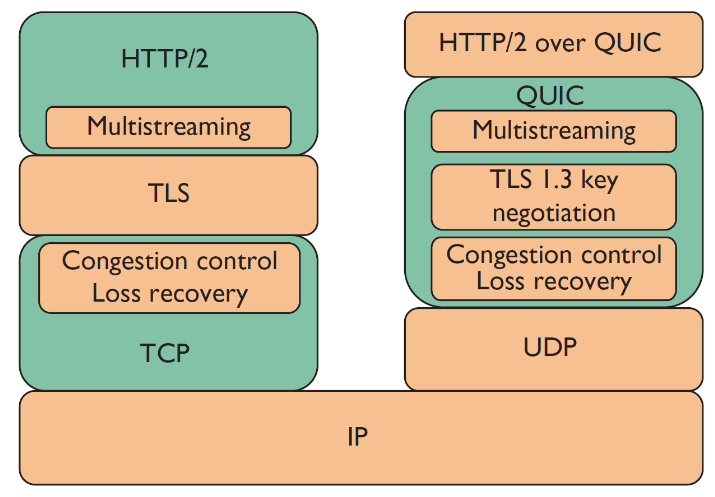
\includegraphics[width=5cm]{quic}
	\end{center}
\end{wrapfigure}
QUIC can be viewed as a \textbf{bidirectional} UDP packet sequence with concealed payload, which is encrypted before getting to the UDP protocol. This means that now more mechanisms are in the user space and it's simpler and faster to update.

\begin{wrapfigure}[9]{r}{5cm}
	\begin{center}
		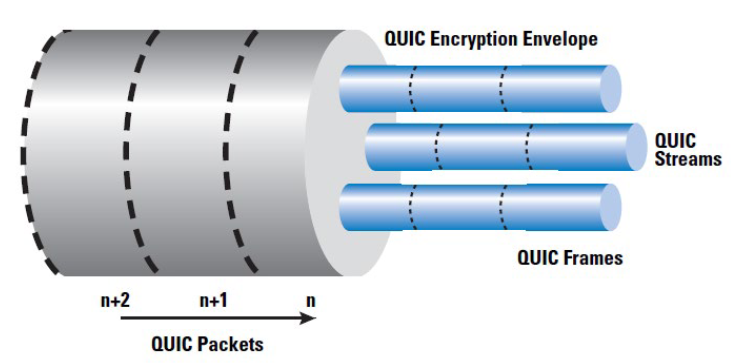
\includegraphics[width=5cm]{quicstream}
	\end{center}
\end{wrapfigure}
\paragraph{Connection} A QUIC connection is identified by a pair of \textbf{ID}s, one for each endpoint: a persistent identity for a connection independent of changes at lower layers (merges the concept of TCP+TLS 1.3).
\paragraph{Packet} QUIC packets are individually $62$bit numbered and cannot be retransmitted using the same one (the next one is used). Multiple packets may form the payload of a UDP datagram with an assumed minimum of $1200$byte (padded if necessary) and without fragmentation.\\
\textbf{Encryption} is based on individual packet, thus avoiding the wait for partially delivered ones.\\
The receiver \textbf{ACK}s the highest packet number received so far and adds a list of received contiguous packet numbers (maximum $256$).

\paragraph{Streams} Each connection contains one ore more streams, which is similar to a TCP one. They may have a priority defined by the application and are identified by an ID, with special bits to identify the initiator and if bi/unidirectional.\\
Stream creation is very \textbf{lightweight} compared to TCP since the QUIC connection is already open: open a stream, send data and close it in a single packed, reducing latency.\\
Streams are then segmented into \textbf{data frames} of $20$ different types, identified with an offset (similar to TCP sequence number), and used for in-order delivery, loss detection and retransmission.

\paragraph{Recovery} Loss detection is based on packets instead of frames. A packet is considered lost if while it's still unACKed a later sent one is ACKed \textbf{and} a lost threshold is met:
\begin{itemize}
	\item Given an ACKed packet $x$, all unACKed packets with number $< x-t$ are considered lost, with $t$ being the \textbf{reordering threshold}
	\item Given the time of the most recent ACK $t$, then all unACKed packets sent before time $t-w$ are considered lost, with $w$ being the \textbf{waiting time}, derived from a weighted estimate RTT
\end{itemize}
Frames of lost packets are then placed in new ones for retransmission.

\paragraph{Flow/Congestion control} Similar to the mechanism of TCP Window: there is a maximum amount of data a sender can send on an individual stream and on all others.

\paragraph{Issues} The main issues with QUIC are:
\begin{itemize}
	\item \textbf{Load-balancing}: load balancers often categorize packets based on protocol and socket pair, which are not stable for the entire QUIC session. Furthermore, high-capacity infrastructures assumes TCP is used for data-streams and not UDP, not allowing optimization.
	\item \textbf{Encryption cost}
	\item \textbf{Firewalls}: not all of them can handle QUIC and some block it
	\item \textbf{Performance}: it depends on the settings and will change over time due to newer implementations but at the moment it's not faster than TCP on most scenarios
\end{itemize}

\subsubsection{SCTP}
\textbf{Stream Control Transmission Protocol} is a reliable, connection-oriented and message-oriented transport protocol. It uses \textbf{heartbeats} and \textbf{4-way-handshake} to support:
\begin{itemize}
	\item \textbf{Multi-streaming}: allows the partitioning of data into multiple streams within a single \textbf{association}. Streams are \textbf{independent} of sequence delivery, meaning that the loss in one stream will only affect its delivery.\\
	Two sequence numbers are used:
	\begin{itemize}
		\item \textbf{Transmission} SN: governs the transmission of messages and detects message losses
		\item \textbf{Stream Identification}/\textbf{Stream} SN: determines the sequence of delivery of received data
	\end{itemize}
	E.g. partial ordering of web page objects: each one is assigned to a stream without caring about delivery order. Even if an object doesn't get through, the others do, improving the user experience.
	\item \textbf{Multi-homing}: ability of a single endpoint to support multiple IP addresses. Used for redundancy: a fail on one network will not cause a failure of the association.\\
	One address is chosen as the \textbf{primary} and it's the destination for all data chunks for normal transmission, while retransmitted data use alternate addresses. A continued failure on the primary address results in transmitting all data to another one until heartbeats can reestablish the primary one.
\end{itemize}
SCTP packets are divided between a \textbf{common header}
\begin{center}
	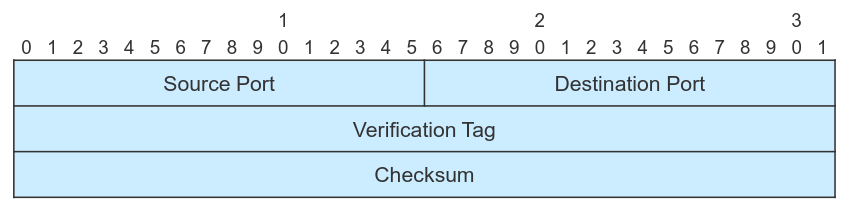
\includegraphics[scale=.3]{sctpheader}
\end{center}
\begin{itemize}
	\item \textbf{Ports}: $16$ bits like TCP and UDP
	\item \textbf{Verification Tag}: validation of the sender, per association. It's set to the value of the Initiate Tag received during association initialization, which is a random number, or set to $0$ in packets with the \textbf{INIT} chunk.
	\item \textbf{Checksum}: CRC32c algorithm using the polynomial
	\begin{equation*}
		x^{32}+x^{28}+x^{27}+x^{26}+x^{25}+x^{23}+x^{22}+x^{20}+x^{19}+x^{18}+x^{14}+x^{13}+x^{11}+x^{10}+x^9+x^8+x^6+1
	\end{equation*}
	and calculated over the whole SCTP packet, including the common header (with checksum value at $0$) and all the chunks.
\end{itemize}
\newpage
and $n$ \textbf{chunks} with the format
\begin{center}
	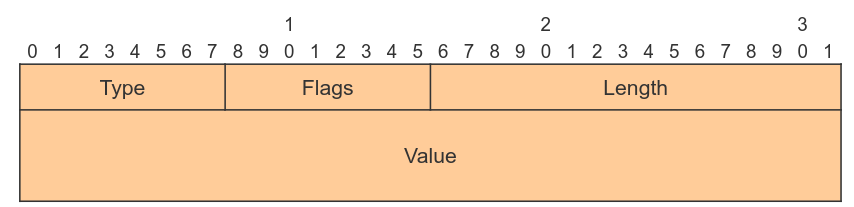
\includegraphics[scale=.3]{sctpchunk}
\end{center}
\begin{itemize}
	\item \textbf{Type}, e.g. \textit{Payload Data} $1$, with its related flags
	\begin{center}
		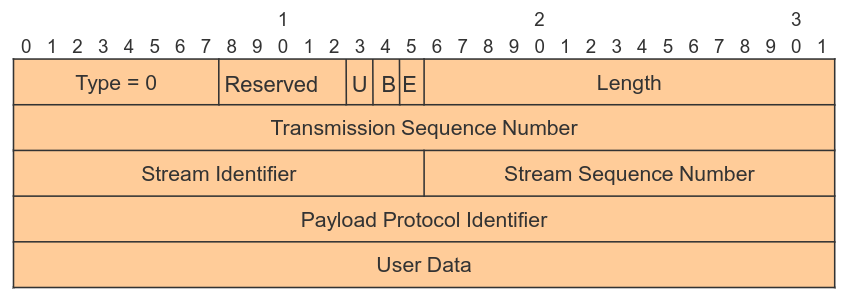
\includegraphics[scale=.2]{stcppayloadchunk}
	\end{center}
	\begin{itemize}
		\item \textbf{U}: unordered data chunk, ignore SSN
		\item \textbf{B} and \textbf{E}
		\begin{table}[!h]
			\centering
			\begin{tabular}{c|c|c}
				\textbf{B} & \textbf{E} & \textbf{Meaning} \\
				\hline
				$1$ & $0$ & First fragment of a user message \\
				\hline
				$0$ & $0$ & Middle fragment of an user message \\
				\hline
				$0$ & $1$ & Last fragment of an user message \\
				\hline
				$1$ & $1$ & Unfragmented user message
			\end{tabular}
		\end{table}
		\item \textbf{Transmission Sequence number}
		\item \textbf{Stream Identifier}: identification of data stream to which the following data belongs
		\item \textbf{Stream Sequence Number}: sequence number of the following user data within the stream, when a user message is fragmented all fragments must carry the same SSN
		\item \textbf{Payload Protocol Identifier}: identifies application layer protocol used by end or intermediate systems
	\end{itemize}
	\item \textbf{Length}: overall length of chunk in bytes
	\item \textbf{Data}: actual content
\end{itemize}